\chapter{Evaluation}

\section{Customer Requirements}

These are the original objectives specified by the client at the analysis stage of making this system.

\textbf{General Objectives}

\begin{itemize}
	\item To have an interactive and easily navigable graphical user interface, applying a suitable colour scheme and layout
	\item To make the database concise and adjustable
	\item To create various lessons, with a wide range of challenges, which effectively teach students how to do trigonometry and Pythagoras
	\item To create tasks which are relevant to the lessons to be completed by the user in order to test their progress
	\item To allow this progress to be recorded in an easily accessible and readable database
	\item To incorporate algorithms which find and/or check the solution given by the user accurately and give clear and easy to read outputs to correspond with said inputs
	\item To have some access restrictions to certain levels of user
	\item To make the program accessible only from various computers with permissions
\end{itemize}

\textbf{Specific Objectives}

\begin{itemize}
	\item To create a teaching program that uses the new GCSE Maths curriculum, as lots of resources will soon be out of date
	\item To include the following topics: Trigonometry, Pythagoras, 3D Trigonometry, 3D Pythagoras
	\item To include a range of difficulty levels, which can challenge every user's level of ability
	\item Use drag and drop, text boxes and drop down menus for inputs
	\item To include interactive 2D graphics which give a clearer idea of the method being shown to the user
	\item To have a database which can be accessed by different computers online
	\item Use a specific, continuous and attractive colour scheme in every window
	\item To have medium sized, highly visible icons
	\item To have all input buttons randomised to avoid double clicking and guessing from memory
	\item To have small error message windows which pop up and disappear on a timer
	\item To include images and shapes which contrast the colour scheme so they are visible and readable
\end{itemize}

\textbf{Core Objectives}

\begin{itemize}
	\item To create a teaching program that uses the new GCSE Maths curriculum, as lots of resources will soon be out of date
	\item To make the database easy to access and easy to read
	\item To include primarily trigonometry based topics, such as how to use the sine, cosine and tan rules
	\item To include an initial, moderate difficulty in order to cater for a majority of students
	\item To make the database functional and able to store the requested details
\end{itemize}

\textbf{Other Objectives}

\begin{itemize}
	\item To position buttons, text boxes and drag and drop boxes in within the layout of the graphical user interface in such a way that cheating and lucky guessing can be minimised
	\item To make the database adjustable if necessary
	\item Use a more interesting range of input types like drawing boxes rather than just clicking and typing
	\item To include a wider range of difficulties to challenge every student on the right level for them
	\item To include a wider range of topics such as Pythagoras, then 3D Trigonometry and 3D Pythagoras
\end{itemize}

\subsection{General Objective 1: }

To have an interactive and easily navigable graphical user interface, applying a suitable colour scheme and layout

\subsubsection{Objective Met?}

This objective has been met. My windows all use a consistent layout which includes large buttons, for easy clicking, and a highly visible colour scheme. Labels make it clear how to navigate to certain parts of the system, and a colour code is used to imply to the user what the purpose of each button is. For example, blue to proceed, red to go back, green to submit/complete something, and yellow to mark an input. Each window has a large title so the user always knows where they are.

\subsubsection{Evidence: }

\begin{figure}[H]
	
\includegraphics{C:/Users/Jordan/git/COMP4Coursework2/Evaluation/objective_1}
\end{figure}

\begin{figure}[H]
	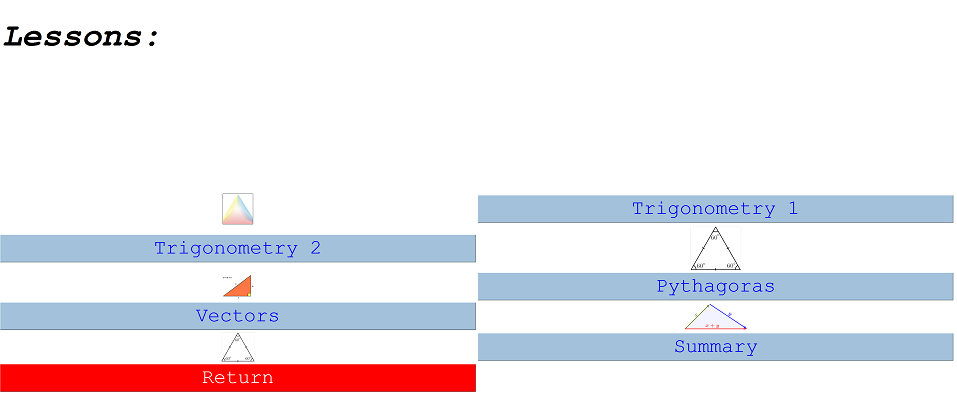
\includegraphics{C:/Users/Jordan/git/COMP4Coursework2/Evaluation/evidence_1_1}
	\caption{This window uses the generic layout and colour scheme....}
\end{figure}

\begin{figure}[H]
	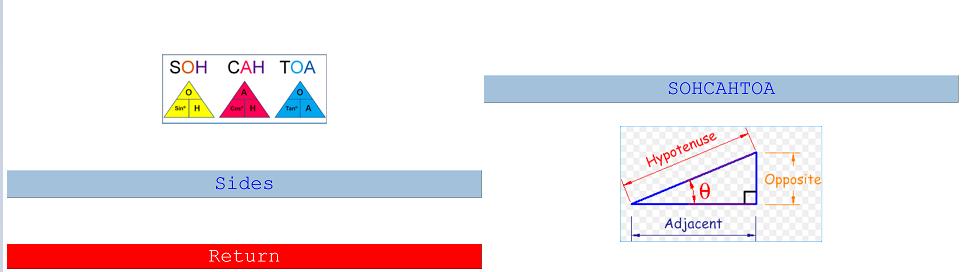
\includegraphics{C:/Users/Jordan/git/COMP4Coursework2/Evaluation/evidence_1_2}
	\caption{...as does this one, and all of the others, making it consistent throughout the system} 
\end{figure}

\subsection{General Objective 2: }

To make the database concise and adjustable

\subsubsection{Objective Met?}

This objective has been met. The database is small, as it only stores five different entities, which technically is a short-coming but for a separate objective. The database is easily visible and the table widget which displays it is designed to fit itself in any sized screen, and scroll bars are available if necessary. The number of rows is hard-coded as there is a maximum number of records that can be recorded in version 1 of the system, and before these records are saved there are just blank spaces in a pre-set table.

\subsubsection{Evidence: }

\begin{figure}[H]
	
\includegraphics{C:/Users/Jordan/git/COMP4Coursework2/Evaluation/objective_2}
\end{figure}

\begin{figure}[H]
	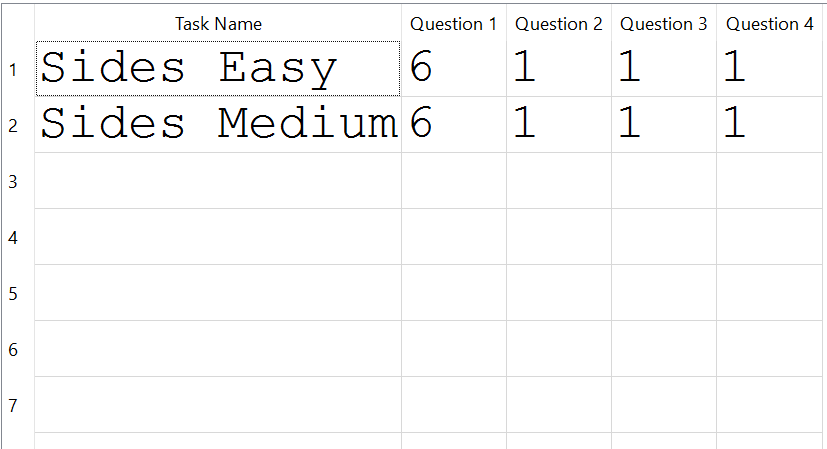
\includegraphics{C:/Users/Jordan/git/COMP4Coursework2/Evaluation/evidence_2}
	\caption{The database only has five entities, and is displayed in a single table widget}
\end{figure}

\subsection{General Objective 3: }

To create various lessons, with a wide range of challenges, which effectively teach students how to do trigonometry and Pythagoras

\subsubsection{Objective Met?}

This objective has been met. There are nine lessons which all cover trigonometry, Pythagoras, or an aspect of either one, as well as some vector lessons.

\subsubsection{Evidence: }

\begin{figure}[H]
	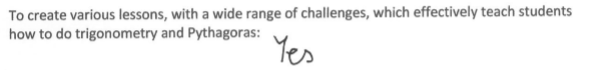
\includegraphics{C:/Users/Jordan/git/COMP4Coursework2/Evaluation/objective_3}
\end{figure}

\begin{figure}[H]
	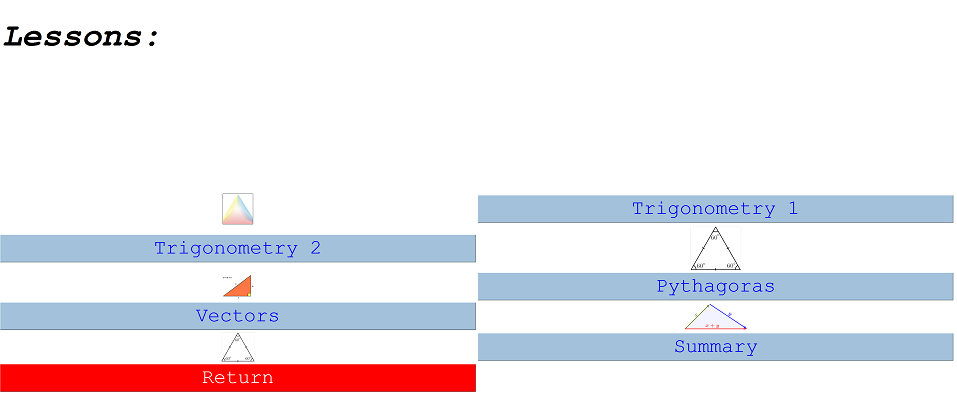
\includegraphics{C:/Users/Jordan/git/COMP4Coursework2/Evaluation/evidence_1_1}
	\caption{The menu which leads to any of the nine lessons, all relevant to trigonometry in some way}
\end{figure}

\subsection{General Objective 4: }

To create tasks which are relevant to the lessons to be completed by the user in order to test their progress

\subsubsection{Objective Met?}

This objective has been met. Each lesson has three homework tasks which are based directly on the content of said lesson, and upon completing each task the user will have a better idea of how good their knowledge of the topic is.

\subsubsection{Evidence: }

\begin{figure}[H]
	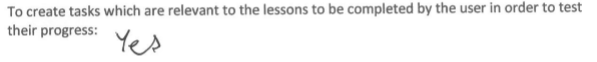
\includegraphics{C:/Users/Jordan/git/COMP4Coursework2/Evaluation/objective_4}
\end{figure}

\begin{figure}[H]
	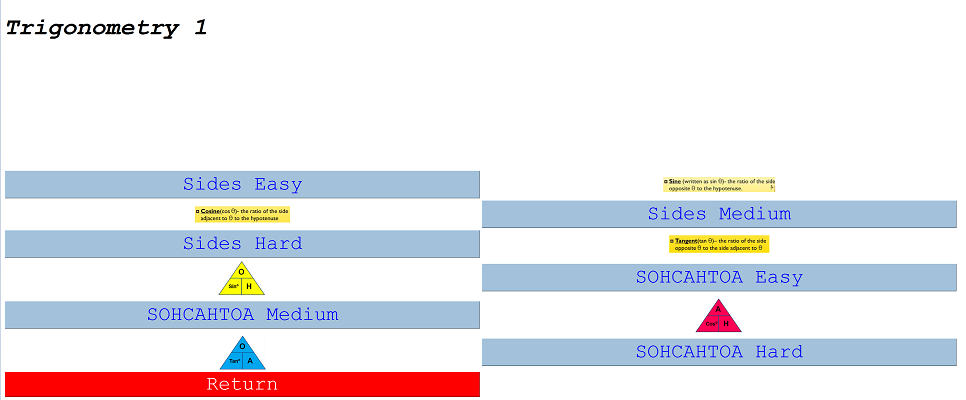
\includegraphics{C:/Users/Jordan/git/COMP4Coursework2/Evaluation/evidence_4}
	\caption{Example of a menu showing all of the homework relevant to some lessons}
\end{figure}

\subsection{General Objective 5: }

To allow this progress to be recorded in an easily accessible and readable database

\subsubsection{Objective Met?}

This objective has been met. There is a table widget accessible from one click on the home screen which, when its window is opened, immediately displays up-to-date information from the database file. The size of the table widget has been altered to make it readable and fit well with most monitor sizes.

\subsubsection{Evidence: }

\begin{figure}[H]
	
\includegraphics{C:/Users/Jordan/git/COMP4Coursework2/Evaluation/objective_5}
\end{figure}

\begin{figure}[H]
	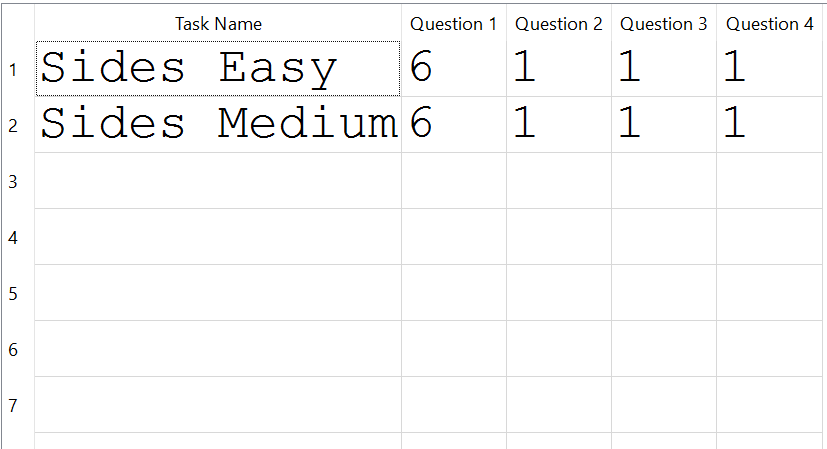
\includegraphics{C:/Users/Jordan/git/COMP4Coursework2/Evaluation/evidence_2}
	\caption{The database information is easy to access from the home screen, displayed in a readable table}
\end{figure}

\subsection{General Objective 6: }

To incorporate algorithms which find and/or check the solution given by the user accurately and give clear and easy to read outputs to correspond with said inputs

\subsubsection{Objective Met?}

This objective has been met. There are various check methods in the parent homework classes which are used to check the value of the user's input, which is passed into the method from the subclass, against a hard-coded answer. The user will be told if they are right or wrong, and error messages prevent them from missing questions.

\subsubsection{Evidence: }

\begin{figure}[H]
	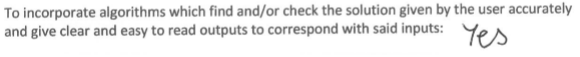
\includegraphics{C:/Users/Jordan/git/COMP4Coursework2/Evaluation/objective_6}
\end{figure}

\begin{figure}[H]
	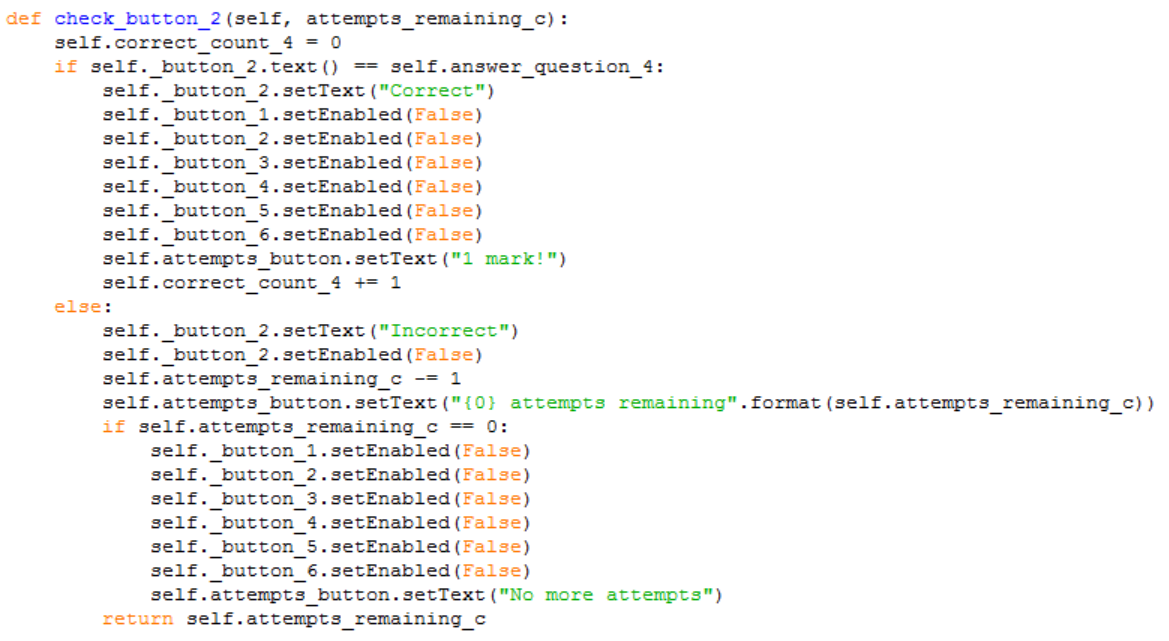
\includegraphics{C:/Users/Jordan/git/COMP4Coursework2/Evaluation/evidence_6}
	\caption{a piece of code/check method which checks the users input and tells them if they are right or not}
\end{figure}

\subsection{General Objective 7: }

To have some access restrictions to certain levels of user

\subsubsection{Objective Met?}

This objective has not been met. This system ended up being a single user, offline program which can only be used by one person per machine, which it has to be installed on. There are no administrator only aspects to the system; every possible user will have the same access to the whole program.

\subsubsection{Evidence: }

\begin{figure}[H]
	
\includegraphics{C:/Users/Jordan/git/COMP4Coursework2/Evaluation/objective_7}
\end{figure}

\begin{figure}[H]
	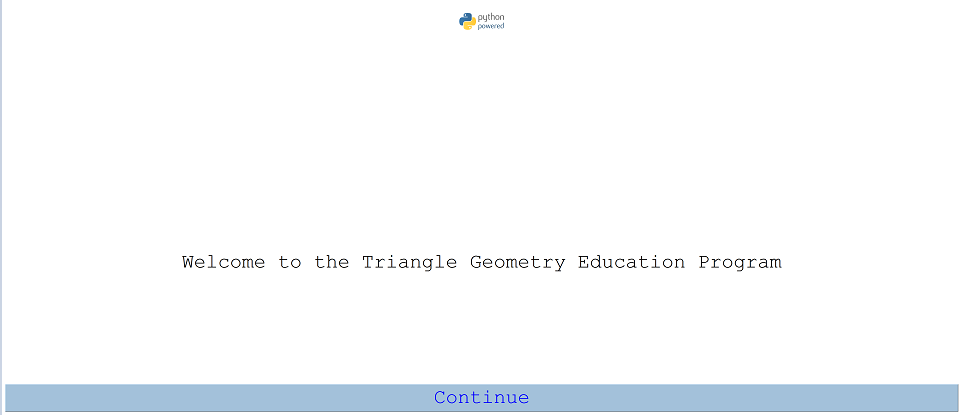
\includegraphics{C:/Users/Jordan/git/COMP4Coursework2/Evaluation/evidence_7}
	\caption{The welcome screen, absent of any log in requests or identity}
\end{figure}

\subsection{General Objective 8: }

To make the program accessible only from various computers with permissions

\subsubsection{Objective Met?}

This objective has been met in one sense, but has not been met in another. To use this program, the installer has to be obtained from me directly, and only the computer which you install it on can use it. There are no restrictions on which computers can use it, as long as it runs on Windows. However, there is no logging in function in the system, so there is no way to know for sure who is using the system of the people who might have access to a computer it is installed on, so effectively this objective has not been met.

\subsubsection{Evidence: }

\begin{figure}[H]
	
\includegraphics{C:/Users/Jordan/git/COMP4Coursework2/Evaluation/objective_8}
\end{figure}

\begin{figure}[H]
	
\includegraphics{C:/Users/Jordan/git/COMP4Coursework2/Evaluation/evidence_8}
	\caption{The application in the task bar - anyone on the computer can use it}
\end{figure}

\subsection{Specific Objective 1: }

To create a teaching program that uses the new GCSE Maths curriculum, as lots of resources will soon be out of date

\subsubsection{Objective Met?}

This objective has not been met. I have included tasks which require the application of skills rather than problem solving tasks, like the current and soon to be out dated curriculum.

\subsubsection{Evidence: }

\begin{figure}[H]
	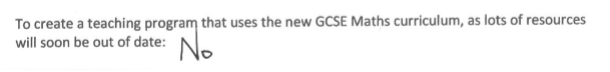
\includegraphics{C:/Users/Jordan/git/COMP4Coursework2/Evaluation/objective_9}
\end{figure}

\begin{figure}[H]
	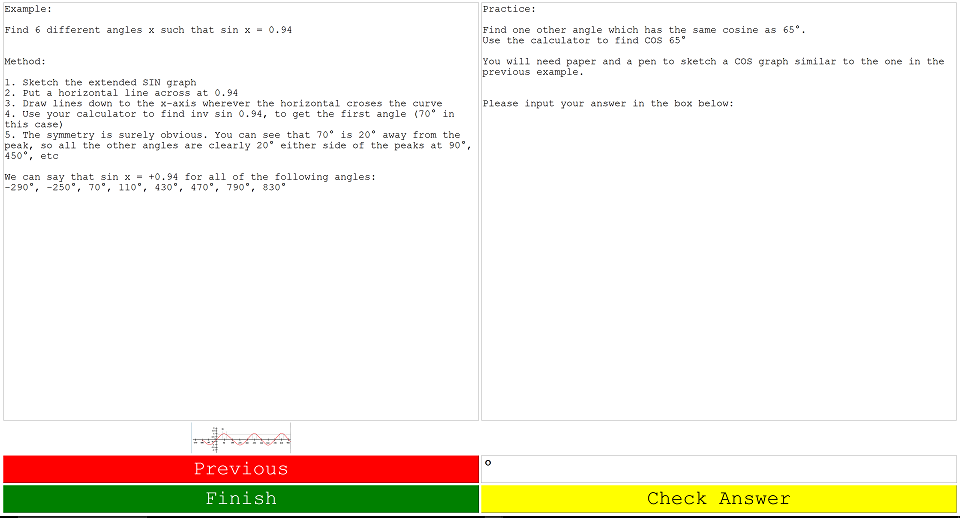
\includegraphics{C:/Users/Jordan/git/COMP4Coursework2/Evaluation/evidence_9}
	\caption{An example of the subject material used, still based on application of skills rather than problem solving}
\end{figure}

\subsection{Specific Objective 2: }

To include the following topics: Trigonometry, Pythagoras, 3D Trigonometry, 3D Pythagoras

\subsubsection{Objective Met?}

This objective has been met. All of the topics listed in the objective have lessons and homework tasks in the system, and other sub topics have been included as well.

\subsubsection{Evidence: }

\begin{figure}[H]
	
\includegraphics{C:/Users/Jordan/git/COMP4Coursework2/Evaluation/objective_10}
\end{figure}

\begin{figure}[H]
	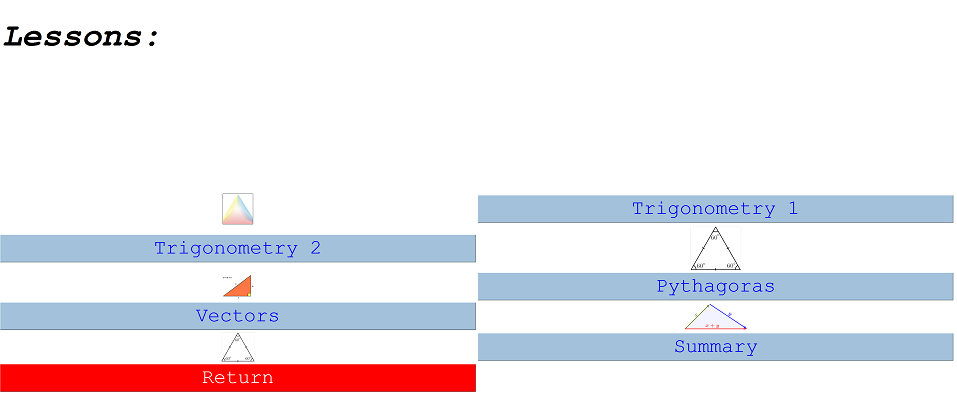
\includegraphics{C:/Users/Jordan/git/COMP4Coursework2/Evaluation/evidence_1_1}
	\caption{A menu which leads to lessons of all of the listed topics}
\end{figure}

\subsection{Specific Objective 3: }

To include a range of difficulty levels, which can challenge every user's level of ability

\subsubsection{Objective Met?}

This objective has been met. Each lesson has three homework tasks which accompany it. One easy one, one medium one and one hard one, so every level of ability can be tested appropriately.

\subsubsection{Evidence: }

\begin{figure}[H]
	
\includegraphics{C:/Users/Jordan/git/COMP4Coursework2/Evaluation/objective_11}
\end{figure}

\begin{figure}[H]
	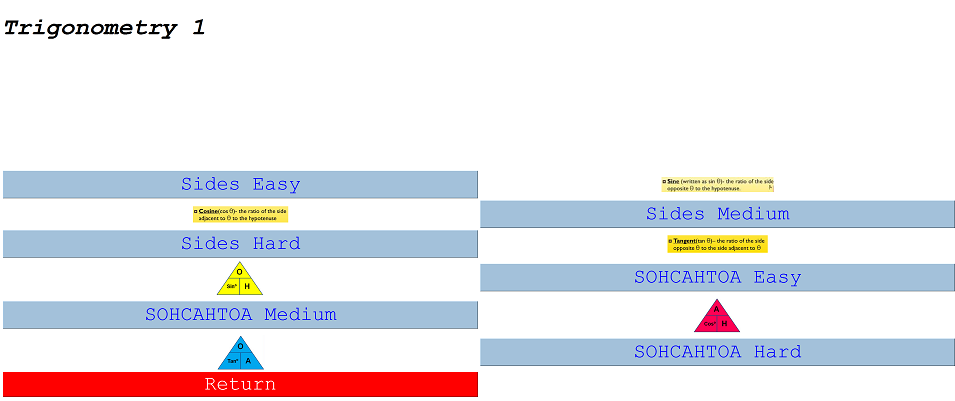
\includegraphics{C:/Users/Jordan/git/COMP4Coursework2/Evaluation/evidence_11}
	\caption{A menu leading to tasks of different difficulty levels}
\end{figure}

\subsection{Specific Objective 4: }

Use drag and drop, text boxes and drop down menus for inputs

\subsubsection{Objective Met?}

This objective has been partially met. Drag and drop functionality was not included, but replaced with multiple choice buttons. Text boxes and drop down menus were included.

\subsubsection{Evidence: }

\begin{figure}[H]
	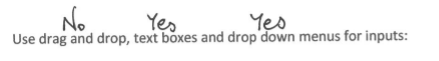
\includegraphics{C:/Users/Jordan/git/COMP4Coursework2/Evaluation/objective_12}
\end{figure}

\begin{figure}[H]
	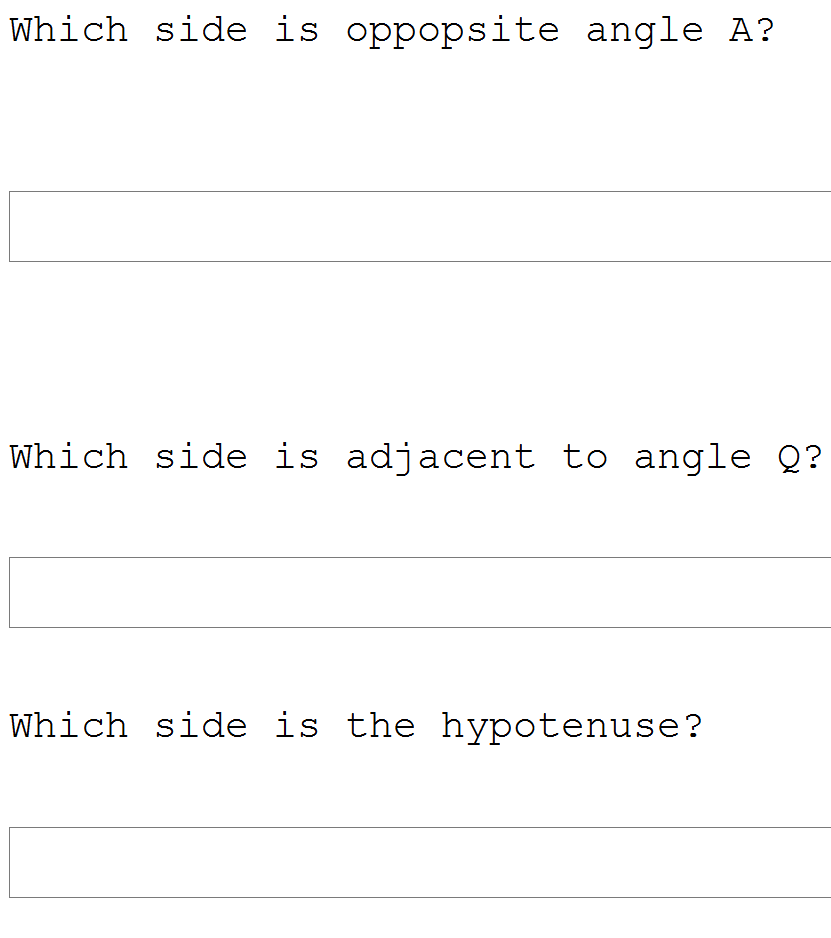
\includegraphics{C:/Users/Jordan/git/COMP4Coursework2/Evaluation/evidence_12_1}
	\caption{An example of line edits in use for text inputs from a keyboard}
\end{figure}

\begin{figure}[H]
	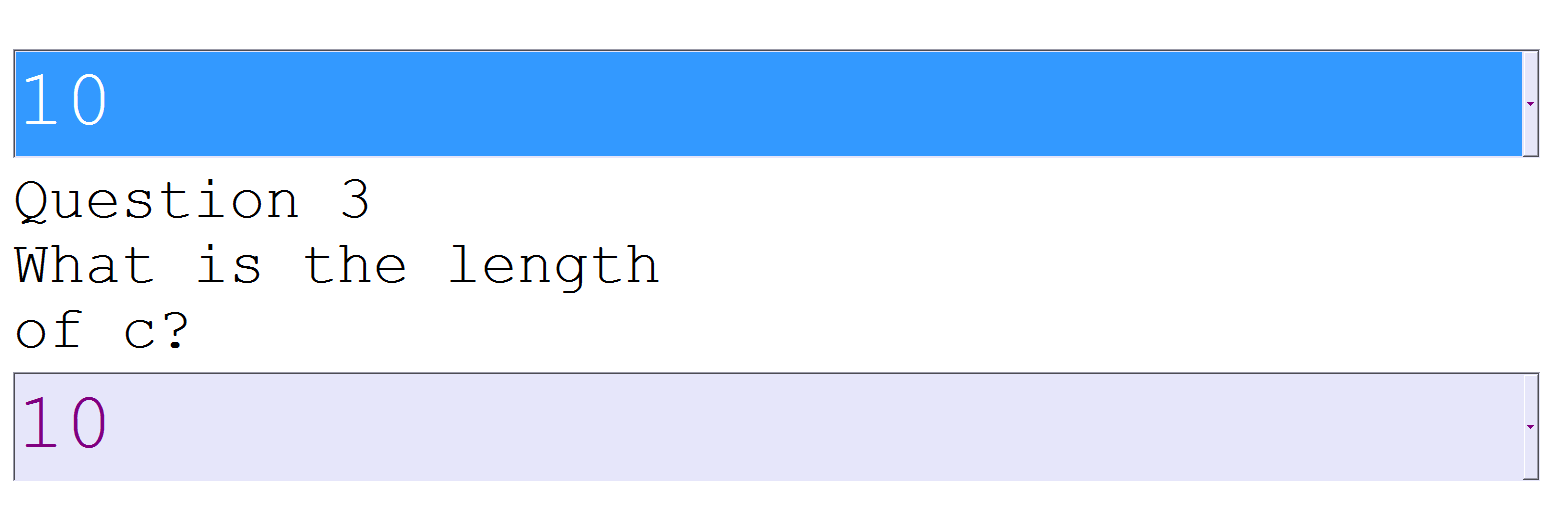
\includegraphics{C:/Users/Jordan/git/COMP4Coursework2/Evaluation/evidence_12_2}
	\caption{An example of the drop down combo boxes}
\end{figure}

\begin{figure}[H]
	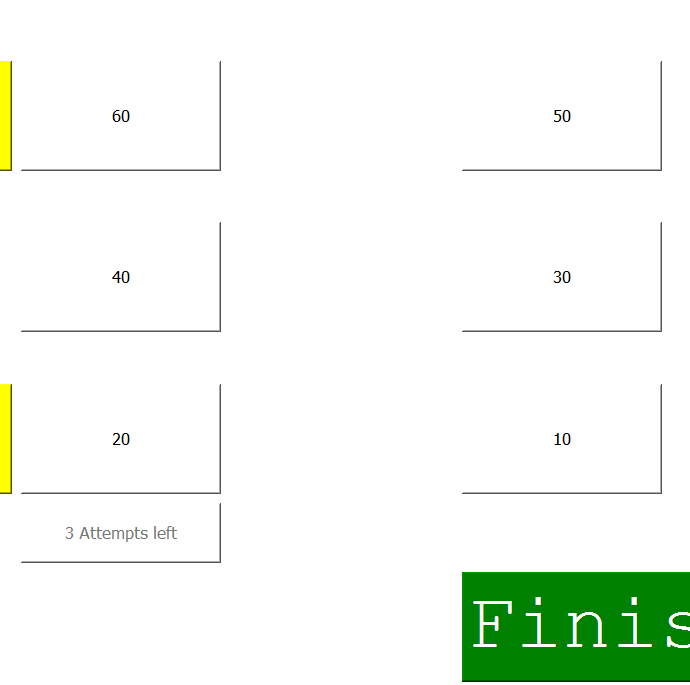
\includegraphics{C:/Users/Jordan/git/COMP4Coursework2/Evaluation/evidence_12_3}
	\caption{An example of the multiple choice button question which replaced the drag and drop input type}
\end{figure}

\subsection{Specific Objective 5: }

To include interactive 2D graphics which give a clearer idea of the method being shown to the user

\subsubsection{Objective Met?}

This objective has been met. Many images have been created (or occasionally taken from Google Images) to provide the user with a better idea of how a method works. However they are not technically interactive, although the user uses some of them to be able to find a solution.

\subsubsection{Evidence: }

\begin{figure}[H]
	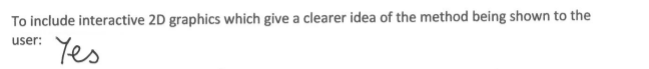
\includegraphics{C:/Users/Jordan/git/COMP4Coursework2/Evaluation/objective_13}
\end{figure}

\begin{figure}[H]
	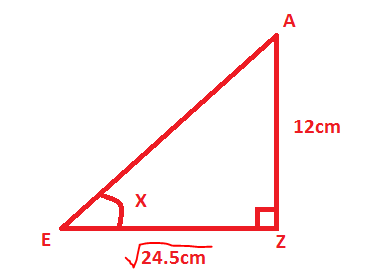
\includegraphics{C:/Users/Jordan/git/COMP4Coursework2/Evaluation/evidence_13}
	\caption{An example of the mathematical diagrams used to show a user how to solve a problem}
\end{figure}

\subsection{Specific Objective 6: }

To have a database which can be accessed by different computers online

\subsubsection{Objective Met?}

This objective has not been met. There is no online functionality at all in this system. Each database is created independently on each individual machine the system is installed on, and can only record the progress of the user who owns the machine.

\subsubsection{Evidence: }

\begin{figure}[H]
	
\includegraphics{C:/Users/Jordan/git/COMP4Coursework2/Evaluation/objective_14}
\end{figure}

\begin{figure}[H]
	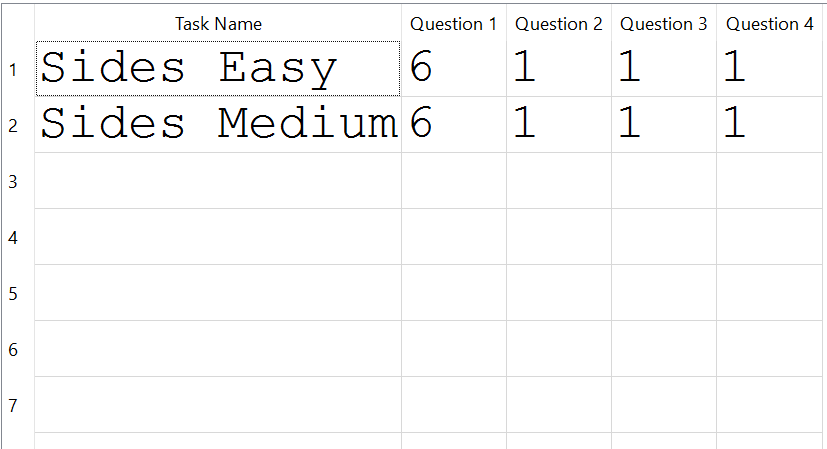
\includegraphics{C:/Users/Jordan/git/COMP4Coursework2/Evaluation/evidence_2}
	\caption{The simple database with no online capabilities whatsoever, just a single user progression recorder}
\end{figure}

\subsection{Specific Objective 7: }

Use a specific, continuous and attractive colour scheme in every window

\subsubsection{Objective Met?}

This objective has been met. The colour scheme is consistent, attractive and has a code, making it specific, and therefore has high usability.

\subsubsection{Evidence: }

\begin{figure}[H]
	
\includegraphics{C:/Users/Jordan/git/COMP4Coursework2/Evaluation/objective_15}
\end{figure}

\begin{figure}[H]
	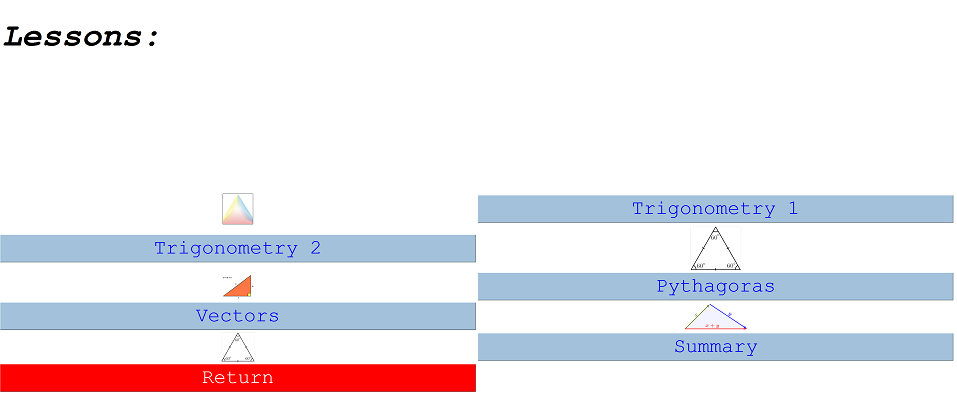
\includegraphics{C:/Users/Jordan/git/COMP4Coursework2/Evaluation/evidence_1_1}
	\caption{Again, the colour scheme is consistent in each window}
\end{figure}

\begin{figure}[H]
	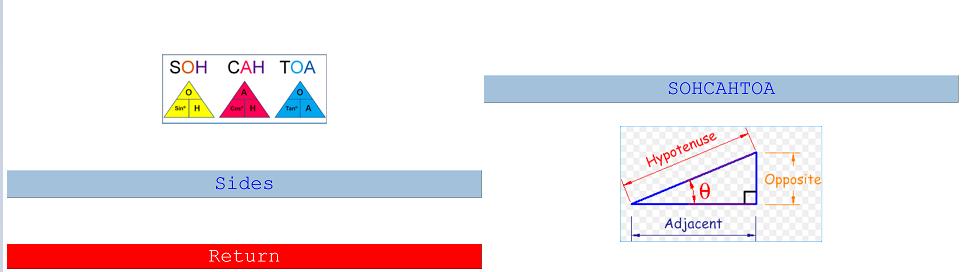
\includegraphics{C:/Users/Jordan/git/COMP4Coursework2/Evaluation/evidence_1_2}
	\caption{It is also kind on the eyes and the colour code is memorable once you figure out what it is}
\end{figure}

\subsection{Specific Objective 8: }

To have medium sized, highly visible icons

\subsubsection{Objective Met?}

This objective has been met. All of the widgets in the system are just the right size, not too big or small. They generally fit well on the screen, as long as the screen is at least 20 inches wide.

\subsubsection{Evidence: }

\begin{figure}[H]
	
\includegraphics{C:/Users/Jordan/git/COMP4Coursework2/Evaluation/objective_16}
\end{figure}

\begin{figure}[H]
	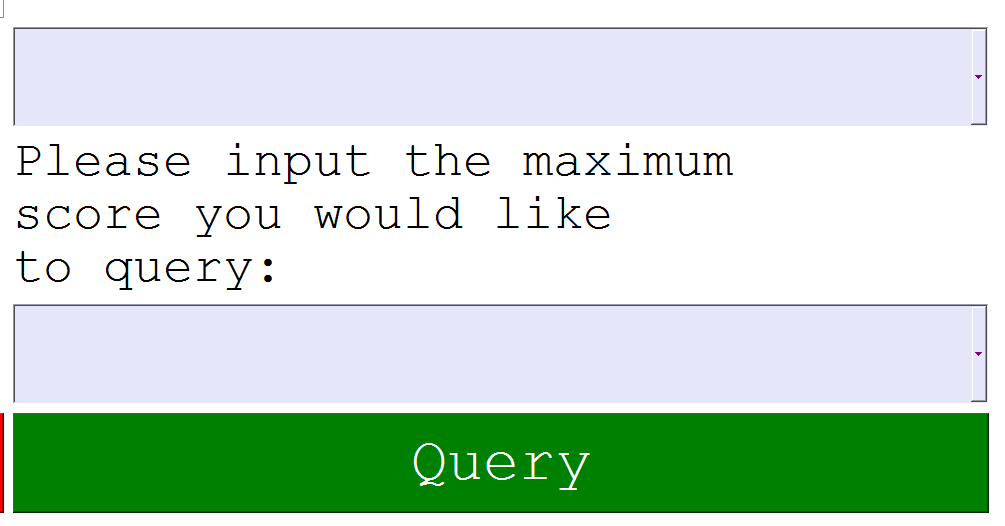
\includegraphics{C:/Users/Jordan/git/COMP4Coursework2/Evaluation/evidence_16}
	\caption{An example of the large widgets used to make it easier for all users to see them and use them quicker}
\end{figure}

\subsection{Specific Objective 9: }

To have all input buttons randomised to avoid double clicking and guessing from memory

\subsubsection{Objective Met?}

This objective has not been met. I could not find a suitable randomisation solution, so the location of each answer will be hard-coded. On the other hand, no two homework task windows which have a similar layout will ever appear together, so there is no chance of accidentally clicking a button on a second screen after a double click.

\subsubsection{Evidence: }

\begin{figure}[H]
	
\includegraphics{C:/Users/Jordan/git/COMP4Coursework2/Evaluation/objective_17}
\end{figure}

\begin{figure}[H]
	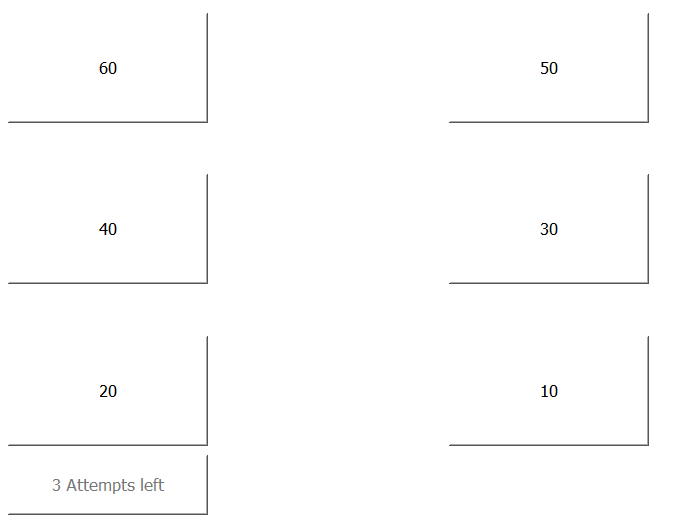
\includegraphics{C:/Users/Jordan/git/COMP4Coursework2/Evaluation/evidence_17}
	\caption{This multiple choice question has buttons with answers displayed on them}
\end{figure}

\begin{figure}[H]
	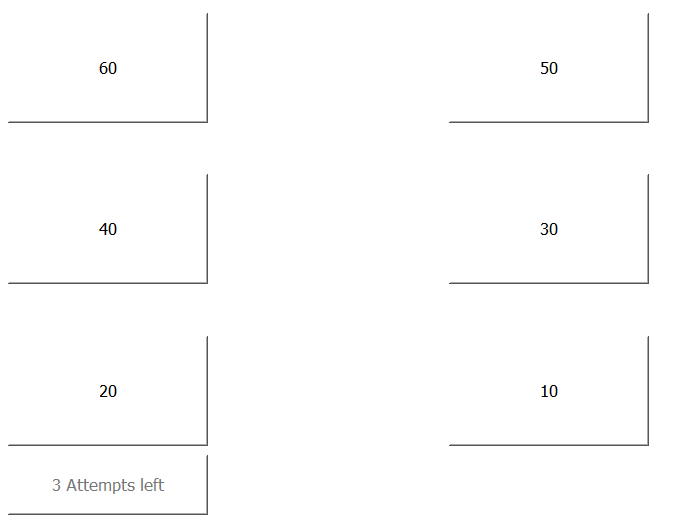
\includegraphics{C:/Users/Jordan/git/COMP4Coursework2/Evaluation/evidence_17}
	\caption{Same question, same answers, same order}
\end{figure}

\subsection{Specific Objective 10: }

To have small error message windows which pop up and disappear on a timer

\subsubsection{Objective Met?}

This objective has been met. Error messages appear at appropriate times to help the user input a correct answer or remind them that they have missed a question.

\subsubsection{Evidence: }

\begin{figure}[H]
	
\includegraphics{C:/Users/Jordan/git/COMP4Coursework2/Evaluation/objective_18}
\end{figure}

\begin{figure}[H]
	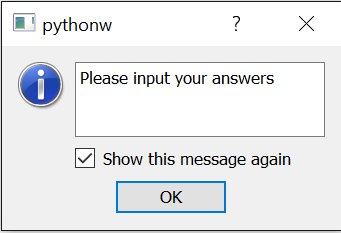
\includegraphics{C:/Users/Jordan/git/COMP4Coursework2/Evaluation/evidence_18}
	\caption{One of the error messages preventing the user from missing a question}
\end{figure}

\subsection{Specific Objective 11: }

To include images and shapes which contrast the colour scheme so they are visible and readable

\subsubsection{Objective Met?}

this objective has been met. The background colour of every window in the system is white, so any colour contrasts it well. Generally the images are of shapes which all have borders, so any white filling will not be mistaken for background.

\subsubsection{Evidence: }

\begin{figure}[H]
	
\includegraphics{C:/Users/Jordan/git/COMP4Coursework2/Evaluation/objective_19}
\end{figure}

\begin{figure}[H]
	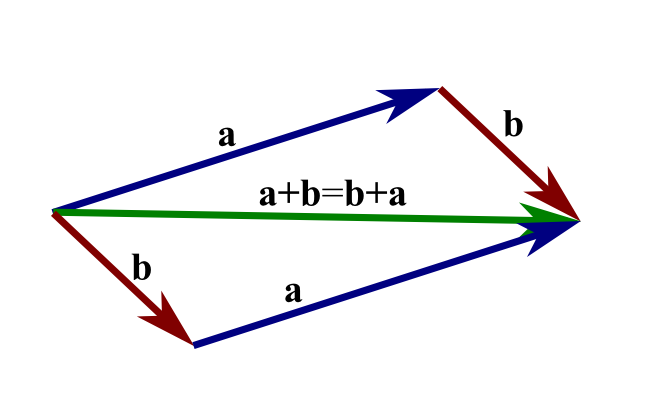
\includegraphics{C:/Users/Jordan/git/COMP4Coursework2/Evaluation/evidence_19}
	\caption{An example of some of the many images included, all of which have good or reasonable resolution}
\end{figure}

\subsection{Core Objective 1: }

To create a teaching program that uses the new GCSE Maths curriculum, as lots of resources will soon be out of date

\subsubsection{Objective Met?}

This objective has not been met. I have included in the system problems which require the application of skills rather than problem solving skills which the new curriculum includes. The subject material is still useful however, even for the new curriculum to an extent.

\subsubsection{Evidence: }

\begin{figure}[H]
	
\includegraphics{C:/Users/Jordan/git/COMP4Coursework2/Evaluation/objective_20}
\end{figure}

\begin{figure}[H]
	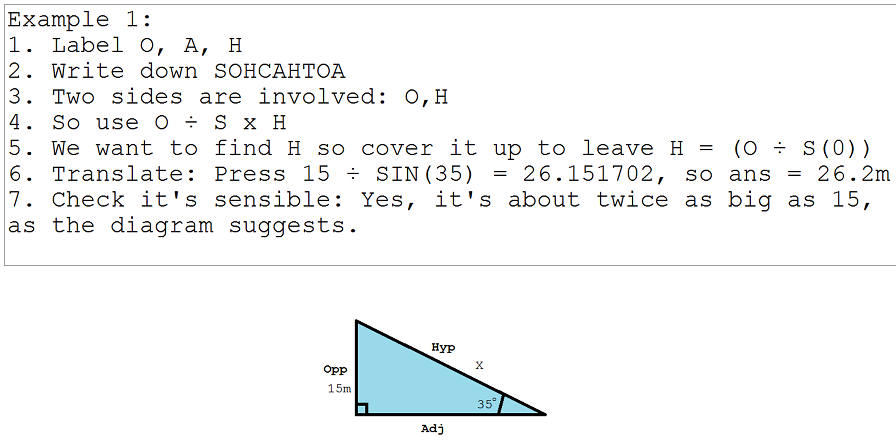
\includegraphics{C:/Users/Jordan/git/COMP4Coursework2/Evaluation/evidence_20}
	\caption{An example of problem solving methods}
\end{figure}

\subsection{Core Objective 2: }

To make the database easy to access and easy to read

\subsubsection{Objective Met?}

This objective has been met. All information in the database is displayed in a table widget which is very easy to access internally, and the text is large and fits well on the screen.

\subsubsection{Evidence: }

\begin{figure}[H]
	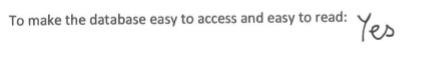
\includegraphics{C:/Users/Jordan/git/COMP4Coursework2/Evaluation/objective_21}
\end{figure}

\begin{figure}[H]
	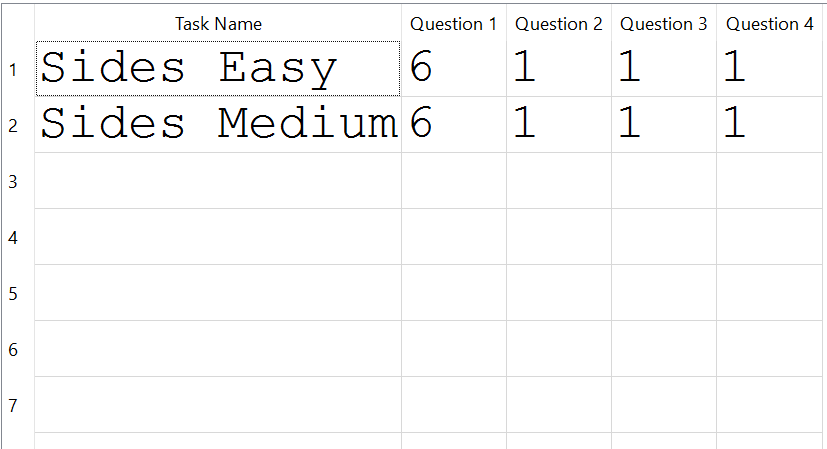
\includegraphics{C:/Users/Jordan/git/COMP4Coursework2/Evaluation/evidence_2}
	\caption{The information from the database being displayed in an easy to read format}
\end{figure}

\subsection{Core Objective 3: }

To include primarily trigonometry based topics, such as how to use the sine, cosine and tan rules

\subsubsection{Objective Met?}

This objective has been met. Subject material covering the majority of GCSE trigonometry has been included in the lessons in the system, as well as the homework which goes with them.

\subsubsection{Evidence: }

\begin{figure}[H]
	
\includegraphics{C:/Users/Jordan/git/COMP4Coursework2/Evaluation/objective_22}
\end{figure}

\begin{figure}[H]
	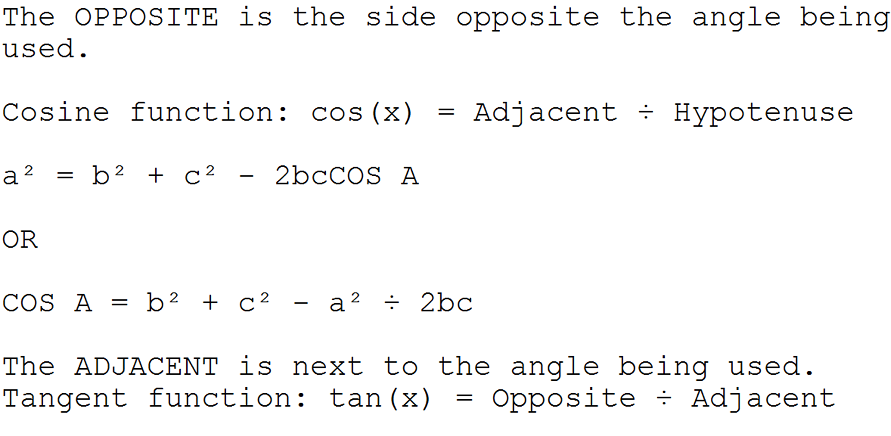
\includegraphics{C:/Users/Jordan/git/COMP4Coursework2/Evaluation/evidence_22}
	\caption{An example of the subject material covered in the system's lessons}
\end{figure}

\subsection{Core Objective 4: }

To include an initial, moderate difficulty in order to cater for a majority of students

\subsubsection{Objective Met?}

This objective has been met. Each lesson has three homework tasks based on the subject material in said lesson. One is easy, one medium and one hard, so every level of ability can be tested.

\subsubsection{Evidence: }

\begin{figure}[H]
	
\includegraphics{C:/Users/Jordan/git/COMP4Coursework2/Evaluation/objective_23}
\end{figure}

\begin{figure}[H]
	\includegraphics{C:/Users/Jordan/git/COMP4Coursework2/Evaluation/evidence_11}
	\caption{A menu showing tasks of varying difficulties}
\end{figure}

\subsection{Core Objective 5: }

To make the database functional and able to store the requested details

\subsubsection{Objective Met?}

This objective has partially been met. The database is functional and stores enough data for a user to gain some idea of how good they are at the maths topics included in the system. However, not all of the entities originally requested by the client are stored in the database.

\subsubsection{Evidence: }

\begin{figure}[H]
	\includegraphics{C:/Users/Jordan/git/COMP4Coursework2/Evaluation/objective_24}
\end{figure}

\begin{figure}[H]
	\includegraphics{C:/Users/Jordan/git/COMP4Coursework2/Evaluation/evidence_2}
	\caption{Only five of the entities originally requested by the user}
\end{figure}

\subsection{Other Objective 1: }

To position buttons, text boxes and drag and drop boxes in within the layout of the graphical user interface in such a way that cheating and lucky guessing can be minimised

\subsubsection{Objective Met?}

This objective has been met. At no point do two similar homework screens appear one after the other, so it is highly unlikely that a double click would accidentally cause a problem by clicking a button on the second screen.

\subsubsection{Evidence: }

\begin{figure}[H]
	\includegraphics{C:/Users/Jordan/git/COMP4Coursework2/Evaluation/objective_25}
\end{figure}

\begin{figure}[H]
	\includegraphics{C:/Users/Jordan/git/COMP4Coursework2/Evaluation/evidence_25_1}
	\caption{The generic first screen of a homework task...}
\end{figure}

\begin{figure}[H]
	\includegraphics{C:/Users/Jordan/git/COMP4Coursework2/Evaluation/evidence_25_2}
	\caption{...always followed by a generic second screen with a completely different layout}
\end{figure}

\subsection{Other Objective 2: }

To make the database adjustable if necessary

\subsubsection{Objective Met?}

This objective has not been met. The user cannot change the database manually at all.

\subsubsection{Evidence: }

\begin{figure}[H]
	\includegraphics{C:/Users/Jordan/git/COMP4Coursework2/Evaluation/objective_26}
\end{figure}

\begin{figure}[H]
	\includegraphics{C:/Users/Jordan/git/COMP4Coursework2/Evaluation/evidence_26}
	\caption{There are no options to amend the database}
\end{figure}

\subsection{Other Objective 3: }

Use a more interesting range of input types like drawing boxes rather than just clicking and typing

\subsubsection{Objective Met?}

This objective has not been met. I could not get a drag and drop functionality to work, so all inputs involve either typing or single clicks.

\subsubsection{Evidence: }

\begin{figure}[H]
	\includegraphics{C:/Users/Jordan/git/COMP4Coursework2/Evaluation/objective_27}
\end{figure}

\begin{figure}[H]
	\includegraphics{C:/Users/Jordan/git/COMP4Coursework2/Evaluation/evidence_12_1}
	\caption{An example of line edits in use for text inputs from a keyboard}
\end{figure}

\begin{figure}[H]
	\includegraphics{C:/Users/Jordan/git/COMP4Coursework2/Evaluation/evidence_12_2}
	\caption{An example of the drop down combo boxes, only using a single click}
\end{figure}

\subsection{Other Objective 4: }

To include a wider range of difficulties to challenge every student on the right level for them

\subsubsection{Objective Met?}

This objective has been met. Each student can choose to begin on an easy or medium task, then if they are comfortable they can try a hard task

\subsubsection{Evidence: }

\begin{figure}[H]
	\includegraphics{C:/Users/Jordan/git/COMP4Coursework2/Evaluation/objective_28}
\end{figure}

\begin{figure}[H]
	\includegraphics{C:/Users/Jordan/git/COMP4Coursework2/Evaluation/evidence_11}
	\caption{A menu showing the range of difficulties of homework tasks}
\end{figure}

\subsection{Other Objective 5: }

To include a wider range of topics such as Pythagoras, then 3D trigonometry and 3D Pythagoras

\subsubsection{Objective Met?}

This objective has been met. All of the topics listed in the objective as well as another topic, vectors, have been included in the system.

\subsubsection{Evidence: }

\begin{figure}[H]
	\includegraphics{C:/Users/Jordan/git/COMP4Coursework2/Evaluation/objective_29}
\end{figure}

\begin{figure}[H]
	\includegraphics{C:/Users/Jordan/git/COMP4Coursework2/Evaluation/evidence_29}
	\caption{A menu showing the range of topics}
\end{figure}

\section{Effectiveness}

\subsection{General Objective 1: }

To have an interactive and easily navigable graphical user interface, applying a suitable colour scheme and layout

\subsubsection{Effective?}

\textbf{Criteria: }

\begin{itemize}
	\item Is the interface readable?
	\item How quickly can the user navigate?
	\item Is the colour scheme suitable?
	\item Is the layout consistent?
	\item Is the interface robust?
\end{itemize}

The graphical user interface I have used in my system is consistent with every window in that it uses the same colour code for widgets, the background, and text. The sizing is the same for pretty much all widgets and images. The widgets are big enough but not too big, so the user can quickly find a button or input box they are looking for, and clearly read the labels which tell the user what the purpose of each widget is. It is quite obvious throughout the system what each widget does due to the large text labelling. The widgets all fit on the screen, and the layout is logical in that the buttons are all level and evenly spaced. Each window is the system can be accessed quickly because there aren't too many windows to go through to find them. The interface is mostly robust; occasionally you have to click twice for a button to work after just having opened a new window, as it has not registered it quickly enough. This occurs for two seconds maximum. Otherwise all of the navigation inputs work fine. There are no bugs or errors, except for those which have error messages if a user misses a question on a homework. Overall, the graphical user interface is effective.

\subsubsection{Evidence}

These images all show different windows using the same colour scheme, widget size and layout.

\begin{figure}[H]
	\includegraphics{C:/Users/Jordan/git/COMP4Coursework2/Evaluation/evidence_1_1}
\end{figure}

\begin{figure}[H]
	\includegraphics{C:/Users/Jordan/git/COMP4Coursework2/Evaluation/evidence_1_2}
\end{figure}

\begin{figure}[H]
	\includegraphics{C:/Users/Jordan/git/COMP4Coursework2/Evaluation/evidence_4}
\end{figure}

\begin{figure}[H]
	\includegraphics{C:/Users/Jordan/git/COMP4Coursework2/Evaluation/evidence_25_1}
\end{figure}

\begin{figure}[H]
	\includegraphics{C:/Users/Jordan/git/COMP4Coursework2/Evaluation/evidence_25_2}
\end{figure}

\subsection{General Objective 2: }

To make the database concise and adjustable

\subsubsection{Effective?}

\textbf{Criteria: }

\begin{itemize}
	\item Is the database concise?
	\item Is the database adjustable?
	\item Is the database easy to use?
\end{itemize}

The table widget where the information from the database can be viewed is concise as it only has five entities in it, and the table fits on the screen well. However, this is technically a short coming as the database does not store all of the entities the client originally requested. Furthermore, the database is not at all adjustable. The user has to delete the entire database file manually from the system files to be able to make a fresh database. They cannot reset any individual task scores. Therefore, this objective is not effective.

\subsubsection{Evidence}

\begin{figure}[H]
	\includegraphics{C:/Users/Jordan/git/COMP4Coursework2/Evaluation/evidence_2}
	\caption{The database is concise, but that wasn't a requirement. If it has more entities it would be effective}
\end{figure}

\subsection{General Objective 3: }

To create various lessons, with a wide range of challenges, which effectively teach students how to do trigonometry and Pythagoras

\subsubsection{Effective?}

\textbf{Criteria: }

\begin{itemize}
	\item Do the lessons include the trigonometry and Pythagoras topics?
	\item Do the lessons contain variation and challenges?
	\item Is the lesson content accurate and effective at teaching students the topic?
\end{itemize}

There are nine lessons, most of which cover a trigonometry or Pythagoras related topic. These lessons are mostly varied (sometimes two separate lessons have content which can be linked), although there aren't many challenges because the lessons are designed to help the user become able to overcome a challenge which is more likely to be in a homework task. The content in the lessons is often detailed and is formatted in a way which makes it easier for the user to read and understand, e.g. spaces between steps in methods. Therefore this objective is moderately effective; this kind of thing can sometimes depend on the user's ability and motivation, although it is possible that some lessons are harder to understand than others. Therefore, this objective is mostly effective.

\subsubsection{Evidence}

\begin{figure}[H]
	\includegraphics{C:/Users/Jordan/git/COMP4Coursework2/Evaluation/evidence_1_1}
	\caption{This menu shows the range of topics}
\end{figure}

\begin{figure}[H]
	\includegraphics{C:/Users/Jordan/git/COMP4Coursework2/Evaluation/evidence_20}
	\caption{This is an example of the content used in the lessons}
\end{figure}

\subsection{General Objective 4: }

To create tasks which are relevant to the lessons to be completed by the user in order to test their progress

\subsubsection{Effective?}

\textbf{Criteria: }

\begin{itemize}
	\item Is the homework relevant to the lessons?
	\item Is the homework useful in helping the user understand the topics better?
	\item Do the homework results give the user an accurate idea of how good they are at the topic?
	\item Is it easy for the user to record and view their progress using the automatic internal database saving functionality?
\end{itemize}

Each lesson has three homework tasks directly related to the lesson content, designed to test the user's new knowledge of the topic. Each is of a different difficulty level so a range of abilities can be tested. The homework results are measured in marks, which generally tend to be single or double. This information is recorded effectively in a database, so the user can see their scores at any time once they complete a task, however due to the lack of the originally requested entities there is not really much to work with to accurately measure your own ability. Furthermore, despite attempts to reduce the opportunities to cheat, it is inevitably possible for the user to guess answers. Therefore, this objective is mostly effective, but it does have its problems.

\subsubsection{Evidence}

\begin{figure}[H]
	\includegraphics{C:/Users/Jordan/git/COMP4Coursework2/Evaluation/evidence_11}
	\caption{This menu shows an example of the homework directly linked to the lessons, with varying difficulties}
\end{figure}

\subsection{General Objective 5: }

To allow this progress to be recorded in an easily accessible and readable database

\subsubsection{Effective?}

\textbf{Criteria: }

\begin{itemize}
	\item Is the progress recorded right?
	\item Is the database easily accessible?
	\item Is the database readable?
\end{itemize}

The progress is always recorded as soon as the user finishes the task, and the answer checking algorithms are effective, so the user can always immediately view the new data in a table by simply clicking a single button once they have finished a task which will open the window with the database table. The text is large and the table itself is designed to fit in most monitor sizes, and there are scroll bars for if the table doesn't fit anyway, so all the data will always be visible. Therefore, the database information is always easy to access and easy to read, so this objective is effective.

\subsubsection{Evidence}

\begin{figure}[H]
	\includegraphics{C:/Users/Jordan/git/COMP4Coursework2/Evaluation/effective_5_1}
	\caption{All of these questions were correct...}
\end{figure}

\begin{figure}[H]
	\includegraphics{C:/Users/Jordan/git/COMP4Coursework2/Evaluation/effective_5_2}
	\caption{...the scores are immediately viewable in the database table}
\end{figure}

\subsection{General Objective 6: }

To incorporate algorithms which find and/or check the solution given by the user accurately and give clear and easy to read outputs to correspond with said inputs

\subsubsection{Effective?}

\textbf{Criteria: }

\begin{itemize}
	\item Do the algorithms check the user's input accurately?
	\item Do the algorithms always give the appropriate output?
	\item Are the algorithms robust?
	\item Do the algorithms work with each subclass?
\end{itemize}

The algorithms always take the text of the input box they have used, so they will always check exactly what the user has input, and the hard-coded answers take into account the special characters like measurements or the {$^0$} symbol. The algorithms will always be able to tell the user whether or not they are correct, and using the appropriate error messages. The algorithms have been tested with each subclass, as they are all written in a parent class, so it will always work, and each task will have data saved in the database once completed. Due to error messages the user will never be able to skip a question, so the values saved in the database will always be accurate. Therefore, this objective is effective.

\subsubsection{Evidence}

\begin{figure}[H]
	\includegraphics{C:/Users/Jordan/git/COMP4Coursework2/Evaluation/effective_5_1}
	\caption{All of these questions were correct and the user was informed they were correct}
\end{figure}

\begin{figure}[H]
	\includegraphics{C:/Users/Jordan/git/COMP4Coursework2/Evaluation/effective_6_2}
	\caption{This question was wrong and an error message popped up to tell the user. The arrow shows were the attempts remaining has decremented}
\end{figure}

\subsection{General Objective 7: }

To have some access restrictions to certain levels of user

\subsubsection{Effective?}

\textbf{Criteria: }

\begin{itemize}
	\item Are there access restrictions in place?
	\item Do the access restrictions work effectively in preventing some users accessing areas of the system?
\end{itemize}

This objective was never implemented, so it is completely ineffective.

\subsubsection{Evidence}

There is no evidence - this objective was never implemented.

\subsection{General Objective 8: }

To make the program accessible only from various computers with permissions

\subsubsection{Effective?}

\textbf{Criteria: }

\begin{itemize}
	\item Are there permission requirements in place?
	\item Is the system only accessible from certain computers?
\end{itemize}

This objective was never implemented, so it is completely ineffective.

\subsubsection{Evidence}

There is no evidence - this objective was never implemented.

\subsection{Specific Objective 1: }

To create a teaching program that uses the new GCSE Maths curriculum, as lots of resources will soon be out of date

\subsubsection{Effective?}

\textbf{Criteria: }

\begin{itemize}
	\item Does the system include material from the up-to-date curriculum?
	\item Does the system include material that is relevant to GCSE maths?
\end{itemize}

The lessons in the system use material which focuses on the application of skills, like the older GCSE maths curriculum, rather than the newer problem solving version of the curriculum, so some of the material in the system may soon go out of date. However, there isn't too much difference between the new and the old versions; this system will still teach users the methods and concepts needed at GCSE level trigonometry, some of which will still be applicable to the new curriculum. Therefore, this objective is partially effective.

\subsubsection{Evidence}

\begin{figure}[H]
	\includegraphics{C:/Users/Jordan/git/COMP4Coursework2/Evaluation/evidence_9}
	\caption{An example of the subject material used in the lessons - corresponds with the current and soon to be replaced curriculum}
\end{figure}

\subsection{Specific Objective 2: }

To include the following topics: Trigonometry, Pythagoras, 3D Trigonometry, 3D Pythagoras

\subsubsection{Effective?}

\textbf{Criteria: }

\begin{itemize}
	\item Is the Trigonometry topic included in the system lessons?
	\item Is the Pythagoras topic included in the system lessons?
	\item Is the 3D Trigonometry topic included in the system lessons?
	\item Is the 3D Pythagoras topic included in the system lessons?
	\item Do the topics included in the system collectively cover the general trigonometry topic thoroughly enough?
\end{itemize}

All of the listed topics have been included in the system lessons. Some are touched on in more than one lesson, and there are other topics covered as well, such as vectors. Collectively, these topics cover everything necessary at GCSE level trigonometry, Pythagoras, and vectors, which is a whole unit in the curriculum. Therefore, this objective is effective.

\subsubsection{Evidence}

\begin{figure}[H]
	\includegraphics{C:/Users/Jordan/git/COMP4Coursework2/Evaluation/evidence_29}
	\caption{This menu shows the range of topics included in the system lessons}
\end{figure}

\subsection{Specific Objective 3: }

To include a range of difficulty levels, which can challenge every user's level of ability

\subsubsection{Effective?}

\textbf{Criteria: }

\begin{itemize}
	\item Is there a range of difficulty levels?
	\item Do these difficulty levels have a wide enough difference to distinguish levels of user skill and allow users of all ability to challenge themselves?
\end{itemize}

Every lesson has three corresponding homework tasks based on the content of the lesson; one is easy, one is medium, and one is hard, so each level of ability can choose to be comfortable or challenge themselves. The difference between difficulties is quite large, so that sometimes a user might not be able to answer a hard question, but will be able to answer a medium question with little difficulty. Therefore, this objective is effective.

\subsubsection{Evidence}

\begin{figure}[H]
	\includegraphics{C:/Users/Jordan/git/COMP4Coursework2/Evaluation/evidence_11}
	\caption{This menu shows the range of difficulty levels of the trigonometry based homework tasks}
\end{figure}

\subsection{Specific Objective 4: }

Use drag and drop, text boxes and drop down menus for inputs

\subsubsection{Effective?}

\textbf{Criteria: }

\begin{itemize}
	\item Has drag and drop functionality been included in the system?
	\item Have text boxes been included in the system?
	\item Have drop down menus been included in the system?
	\item Is there a wide range of input types to make the system more varied?
	\item Can inputs be used quickly and efficiently?
\end{itemize}

Text boxes and drop down menus have been included in the system, but drag and drop functionality has not. Instead multiple choice buttons were included. As a result, the only two hardware inputs are typing and single clicks, so the range of input types is small and potentially boring. None the less, these inputs are always quick and effective; there is no lag or delay, and the buttons to mark the answer are quick too. Overall, due to the absence of drag and drop functionality, this objective is only partially effective, but it is sufficient for the user to use the system easily.

\subsubsection{Evidence}

\begin{figure}[H]
	\includegraphics{C:/Users/Jordan/git/COMP4Coursework2/Evaluation/effective_5_1}
	\caption{An example of the drop down inputs}
\end{figure}

\begin{figure}[H]
	\includegraphics{C:/Users/Jordan/git/COMP4Coursework2/Evaluation/evidence_12_3}
	\caption{An example of the multiple choice buttons which replaced the drag and drop functionality}
\end{figure}

\begin{figure}[H]
	\includegraphics{C:/Users/Jordan/git/COMP4Coursework2/Evaluation/evidence_12_1}
	\caption{An example of the text box inputs}
\end{figure}

\subsection{Specific Objective 5: }

To include interactive 2D graphics which give a clearer idea of the method being shown to the user

\subsubsection{Effective?}

\textbf{Criteria: }
	
\begin{itemize}
	\item Are 2D graphics included in the system?
	\item How high is the resolution of these graphics?
	\item Are the graphics used relevant to the screen they are on?
	\item Are the graphics interactive?
\end{itemize}

2D images from both Google Images and manually drawn in Paint have been included in the system. The resolution of most of the images is high as they have been screen-shotted using Snipping tool. All of the images are entirely relevant to the screen they are on, for example a picture of a vector problem next to the vector button on a menu, or a picture showing how a method is done using the same measurements as the text in the example. Unfortunately, none of the pictures are interactive, although they are useful for the user off screen to use for sketches on paper, if that is how they learn new methods. Therefore, this objective is partially effective as the images are there, and relevant, but not interactive.

\subsubsection{Evidence}

\begin{figure}[H]
	\includegraphics{C:/Users/Jordan/git/COMP4Coursework2/Evaluation/evidence_20}
	\caption{An example of a picture of a method using the same measurements as the text explanation}
\end{figure}

\subsection{Specific Objective 6: }

To have a database which can be accessed by different computers online

\subsubsection{Effective?}

\textbf{Criteria: }

\begin{itemize}
	\item Is there a functional database?
	\item Does the system support online functionality for the database?
\end{itemize}

There is a functional database, however no online functionality was implemented, so this objective is completely ineffective.

\subsubsection{Evidence}

There is no evidence for this objective - it was never implemented.

\subsection{Specific Objective 7: }

Use a specific, continuous and attractive colour scheme in every window

\subsubsection{Effective?}

\textbf{Criteria: }

\begin{itemize}
	\item Is there a colour scheme specifically designed for this system?
	\item Is the colour scheme used throughout the system continuous and appropriate?
	\item Is the colour scheme used throughout the system attractive?
\end{itemize}

There is a colour scheme designed specifically for this system; blue means to continue, red means to return, yellow means to check, purple means to choose, and green means to submit or complete. The background of each window is white, so any colour contrasts it well. The colour scheme is used in every window, and it is attractive and appropriate; pleasant solid block colours used for a system with younger users. This objective is effective.

\subsubsection{Evidence}

These pictures show a few of the windows, all using the same colour scheme:

\begin{figure}[H]
	\includegraphics{C:/Users/Jordan/git/COMP4Coursework2/Evaluation/evidence_1_1}
\end{figure}

\begin{figure}[H]
	\includegraphics{C:/Users/Jordan/git/COMP4Coursework2/Evaluation/evidence_1_2}
\end{figure}

\begin{figure}[H]
	\includegraphics{C:/Users/Jordan/git/COMP4Coursework2/Evaluation/evidence_4}
\end{figure}

\begin{figure}[H]
	\includegraphics{C:/Users/Jordan/git/COMP4Coursework2/Evaluation/evidence_25_2}
\end{figure}

\subsection{Specific Objective 8: }

To have medium sized, highly visible icons

\subsubsection{Effective?}

\textbf{Criteria: }

\begin{itemize}
	\item Are the icons of an appropriate size?
	\item Do the icons fit in a screen of any size?
	\item are the icons visible?
\end{itemize}

The icons/widgets used throughout this system are all sized the same. They are a nice size to be clearly visible and look nice without being too big and excessive. They all fit on a screen of twenty inches wide or bigger, which is the average size of a school standard monitor. The icons are very visible; the colour scheme makes it clear what the purpose of each widget is, and they are all labelled to some degree, so the user can see what they do exactly. Therefore, this objective is effective.

\subsubsection{Evidence}

\begin{figure}[H]
	\includegraphics{C:/Users/Jordan/git/COMP4Coursework2/Evaluation/evidence_9}
	\caption{An example of the icons/widgets used, all labelled appropriately}
\end{figure}

\subsection{Specific Objective 9: }

To have all input buttons randomised to avoid double clicking and guessing from memory

\subsubsection{Effective?}

\textbf{Criteria: }

\begin{itemize}
	\item Are the multiple choice buttons in a randomised order?
	\item Do the buttons appear in a different order to prevent position memorisation?
\end{itemize}

A randomisation method could not be implemented into the classes, so the buttons will appear in the same place every time. Therefore, this objective is not effective.

\subsubsection{Evidence}

\begin{figure}[H]
	\includegraphics{C:/Users/Jordan/git/COMP4Coursework2/Evaluation/evidence_12_3}
	\caption{The buttons when a window is opened}
\end{figure}

\begin{figure}[H]
	\includegraphics{C:/Users/Jordan/git/COMP4Coursework2/Evaluation/evidence_12_3}
	\caption{The buttons when the same window is opened again - in the same place}
\end{figure}

\subsection{Specific Objective 10: }

To have small error message windows which pop up and disappear on a timer

\subsubsection{Effective?}

\textbf{Criteria: }

\begin{itemize}
	\item Are there error messages in place to assist the user?
	\item Do the error messages appear at the appropriate time?
	\item Do the error messages disappear on a timer?
\end{itemize}

There are many error messages in place to assist the user. They tell the user if they are wrong, or have missed a question. They always appear at the appropriate time because they each have a separate class which is called in the appropriate method. They are not on a timer to disappear, however, which goes against the objective, although could be more useful should the user need more time to read them. Therefore, this objective is generally effective.

\subsubsection{Evidence}

\begin{figure}[H]
	\includegraphics{C:/Users/Jordan/git/COMP4Coursework2/Evaluation/evidence_18}
	\caption{An error message appearing to prevent the user from missing a question, dismissible at the user's own pace}
\end{figure}

\subsection{Specific Objective 11: }

To include images and shapes which contrast the colour scheme so they are visible and readable

\subsubsection{Effective?}

\textbf{Criteria: }

\begin{itemize}
	\item Have images and/or shapes been included?
	\item Do these images and/or shapes contrast the colour scheme?
	\item Are these images and/or shapes generally visible?
\end{itemize}

Shapes in the form of images have been included which are relevant to another widget or help to explain a mathematical method. The background is always white so as long as the shapes and images have borders of colour, which they all do, they are visible. Therefore, this objective is effective as all images can be seen and are relevant to a task or widget.

\subsubsection{Evidence}

\begin{figure}[H]
	\includegraphics{C:/Users/Jordan/git/COMP4Coursework2/Evaluation/evidence_13}
	\caption{Example of a shape image against the background, clearly visible}
\end{figure}

\subsection{Core Objective 1: }

To create a teaching program that uses the new GCSE Maths curriculum, as lots of resources will soon be out of date

\subsubsection{Effective?}

\textbf{Criteria: }

\begin{itemize}
	\item Does the system include material from the up-to-date curriculum?
	\item Does the system include material that is relevant to GCSE maths?
\end{itemize}

The lessons in the system use material which focuses on the application of skills, like the older GCSE maths curriculum, rather than the newer problem solving version of the curriculum, so some of the material in the system may soon go out of date. However, there isn't too much difference between the new and the old versions; this system will still teach users the methods and concepts needed at GCSE level trigonometry, some of which will still be applicable to the new curriculum. Therefore, this objective is partially effective.

\subsubsection{Evidence}

\begin{figure}[H]
	\includegraphics{C:/Users/Jordan/git/COMP4Coursework2/Evaluation/evidence_9}
	\caption{An example of the subject material used in the lessons - corresponds with the current and soon to be replaced curriculum}
\end{figure}

\subsection{Core Objective 2: }

To make the database easy to access and easy to read

\subsubsection{Effective?}

\textbf{Criteria: }

\begin{itemize}
	\item How quickly can the database be accessed?
	\item How easy to read is the information in the database?
\end{itemize}

The database can be accessed very quickly by just clicking on the progress button from the home screen. A window will immediately appear with a table displaying the contents of the database in large text, so it is readable too. The information displayed in the database is always refreshed whenever the screen is opened, so it will always be up to date. Therefore, this objective has been met.

\subsubsection{Evidence}

\begin{figure}[H]
	\includegraphics{C:/Users/Jordan/git/COMP4Coursework2/Evaluation/evidence_2}
	\caption{The database - large readable text and accessible from the home screen}
\end{figure}

\subsection{Core Objective 3: }

To include primarily trigonometry based topics, such as how to use the sine, cosine and tan rules

\subsubsection{Effective?}

\textbf{Criteria: }

\begin{itemize}
	\item Are trigonometry based topics the primary topic of the system?
	\item Have the example sub topics been included?
\end{itemize}

There are two sections on trigonometry, and only one on Pythagoras and one on vectors, with a summary section on all of them together, so trigonometry is the main topic included in the system. Furthermore, Pythagoras and vectors also involve trigonometry to some degree. The topics of how to use the sine, cosine and tan rules have been included, as well as all of the other aspects of GCSE level trigonometry. Therefore, this objective is effective.

\subsubsection{Evidence}

\begin{figure}[H]
	\includegraphics{C:/Users/Jordan/git/COMP4Coursework2/Evaluation/evidence_29}
	\caption{This menu shows the range of topics including primarily trigonometry}
\end{figure}

\begin{figure}[H]
	\includegraphics{C:/Users/Jordan/git/COMP4Coursework2/Evaluation/evidence_22}
	\caption{This is part of the lesson which explains the sine, cosine and tan rules}
\end{figure}

\subsection{Core Objective 4: }

To include an initial, moderate difficulty in order to cater for a majority of students

\subsubsection{Effective?}

\textbf{Criteria: }

\begin{itemize}
	\item Is there a default difficulty level?
	\item Can all users find a task at their level of ability?
\end{itemize}

The lessons themselves are of a moderate difficulty; they are not designed to challenge the users, but help prepare them for the challenges in the homework tasks of easy to harder levels. Therefore, this objective is effective, as all users should start by using the lessons.

\subsubsection{Evidence}

\begin{figure}[H]
	\includegraphics{C:/Users/Jordan/git/COMP4Coursework2/Evaluation/evidence_9}
	\caption{The subject material here explains a method to the user and is formatted in an easy to read and understand way}
\end{figure}

\subsection{Core Objective 5: }

To make the database functional and able to store the requested details

\subsubsection{Effective?}

\textbf{Criteria: }

\begin{itemize}
	\item Is the database functional?
	\item Does the database store the requested details?
\end{itemize}

The database is functional, but it does not store all of the requested details. Only enough for the system to serve a basic purpose of allowing the users to broadly keep track of their progress. Therefore, this objective is not effective.

\subsubsection{Evidence}

\begin{figure}[H]
	\includegraphics{C:/Users/Jordan/git/COMP4Coursework2/Evaluation/evidence_2}
	\caption{The database only stores five entities, enough for the user to have a rough idea of their ability level}
\end{figure}

\subsection{Other Objective 1: }

To position buttons, text boxes and drag and drop boxes in within the layout of the graphical user interface in such a way that cheating and lucky guessing can be minimised

\subsubsection{Effective?}

\textbf{Criteria: }

\begin{itemize}
	\item Have the widgets been positioned differently in each subclass?
	\item Are the layouts of the two homework windows in a stack different?
	\item Have the layouts been designed in a way which ultimately reduces or cancels lucking guessing?
\end{itemize}

Each subclass is the same, so it might be easier to remember the answers to some questions, or it might be harder for some people because they all look similar. The first homework screen layout is completely different to the second homework screen layout, so it is unlikely that a double click will get a user an accidental mark, an if they accidentally click finish then an error message will prevent them from closing the stack window. Generally, it is unlikely that the user will accidentally click a button to an irreversible end, however, with all systems like this, it is inevitably possible for the user to make a lucky guess. Therefore, this objective is only partially effective.

\subsubsection{Evidence}

\begin{figure}[H]
	\includegraphics{C:/Users/Jordan/git/COMP4Coursework2/Evaluation/evidence_25_1}
	\caption{This is the generic first homework screen}
\end{figure}

\begin{figure}[H]
	\includegraphics{C:/Users/Jordan/git/COMP4Coursework2/Evaluation/evidence_25_2}
	\caption{The second homework screen uses a different layout}
\end{figure}

\subsection{Other Objective 2: }

To make the database adjustable if necessary

\subsubsection{Effective?}

\textbf{Criteria: }

\begin{itemize}
	\item Is the database adjustable?
\end{itemize}

The database is not adjustable at all. The user just has to stick with their first progress record or delete it entirely manually. This objective is not effective.

\subsubsection{Evidence}

\begin{figure}[H]
	\includegraphics{C:/Users/Jordan/git/COMP4Coursework2/Evaluation/evidence_26}
	\caption{There are no options to adjust the database}
\end{figure}

\subsection{Other Objective 3: }

Use a more interesting range of input types like drawing boxes rather than just clicking and typing

\subsubsection{Effective?}

\textbf{Criteria: }

\begin{itemize}
	\item Have alternative input types been used other than clicking and typing?
	\item Do these input types provide a wider range of input overall?
\end{itemize}

Only clicking and typing inputs were used. Drag and drop functionality could not be implemented and drawing boxes were not used. This limits the range of input types severely, so this objective is not effective.

\subsubsection{Evidence}

\begin{figure}[H]
	\includegraphics{C:/Users/Jordan/git/COMP4Coursework2/Evaluation/evidence_16}
	\caption{An example of a drop down menu, which only requires clicking from the mouse}
\end{figure}

\begin{figure}[H]
	\includegraphics{C:/Users/Jordan/git/COMP4Coursework2/Evaluation/evidence_17}
	\caption{Again, the buttons only require clicking from the mouse, there is no drag and drop functionality for variation}
\end{figure}

\subsection{Other Objective 4: }

To include a wider range of difficulties to challenge every student on the right level for them

\subsubsection{Effective?}

\textbf{Criteria: }

\begin{itemize}
	\item Is there a range of difficulty levels?
	\item Do these difficulty levels have a wide enough difference to distinguish levels of user skill and allow users of all ability to challenge themselves?
\end{itemize}

Every lesson has three corresponding homework tasks based on the content of the lesson; one is easy, one is medium, and one is hard, so each level of ability can choose to be comfortable or challenge themselves. The difference between difficulties is quite large, so that sometimes a user might not be able to answer a hard question, but will be able to answer a medium question with little difficulty. Therefore, this objective is effective.

\subsubsection{Evidence}

\begin{figure}[H]
	\includegraphics{C:/Users/Jordan/git/COMP4Coursework2/Evaluation/evidence_11}
	\caption{This menu shows the range of difficulty levels of the trigonometry based homework tasks}
\end{figure}

\subsection{Other Objective 5: }

To include a wider range of topics such as Pythagoras, then 3D trigonometry and 3D Pythagoras

\subsubsection{Effective?}

\textbf{Criteria: }

\begin{itemize}
	\item Has the Pythagoras topic been included?
	\item Has the 3D Trigonometry topic been included?
	\item Has the 3D Pythagoras topic been included?
	\item Have any other topics been included?
\end{itemize}

All of the topics listed, as well as vectors, have been included in the lessons in the system. Therefore, this objective is effective, as it provides users with a wider range of subject material.

\subsubsection{Evidence}

\begin{figure}[H]
	\includegraphics{C:/Users/Jordan/git/COMP4Coursework2/Evaluation/evidence_29}
	\caption{This menu shows the range of topics included in the system}
\end{figure}

\section{Learnability}

When I first consulted my client I took into account how much experience they have already had using software such as my system. They are comfortable using the internet, so with the assistance of the user manual they should have no problem installing Python 3.4 and PyQt4. They, along with the other people the client intends to use this system with, have all had experience using similar educational maths programs, such as My Maths, which have essentially the same purpose as my system. Therefore, I tried to make some aspects of the system somewhat similar to the ones conventionally used in educational maths programs, such as the layout, including the navigation of the system, the topics, and the rules of saving and popping error messages, such as making sure all questions have been attempted. None the less, this system would probably be easy enough for less experienced users anyway, as generally the buttons are clearly labelled, appropriately sized, and organised in a convenient way (branch menu). Although some users may have issues finding the exact right topic in the sub-menus, being a reason for the big red return buttons which make it easy to go back and try another menu.

\begin{figure}[H]
	\includegraphics{C:/Users/Jordan/git/COMP4Coursework2/Evaluation/learnability_1}
	\caption{An example of the return buttons used to make navigating the sub-menus easier}
\end{figure}

When designing the system I kept in mind the fact that saving data can be a more complex function if it is done manually, especially by an inexperienced user, so I made all of the database functions automatic; they occur when the user simply clicks a button to finish a homework, or opens the progress screen. This cancels out the need for users to learn new skills which they might not have already learned from using similar systems.

\begin{figure}[H]
	\includegraphics{C:/Users/Jordan/git/COMP4Coursework2/Evaluation/learnability_2}
	\caption{The finish button being clicked to automatically save progress for the user}
\end{figure}

\begin{figure}[H]
	\includegraphics{C:/Users/Jordan/git/COMP4Coursework2/Evaluation/learnability_3}
	\caption{The record which was just saved immediately being updated to the database}
\end{figure}

I also endeavoured to make the database itself very easy to access and understand internally in the system; the system accesses the information from a separate file and displays it in a window in the program, which can be accessed by the user very quickly from the home screen, and even queried for specific details should the user be searching for a specific record. the options in the combo boxes are as clear as I can make them to make it easier for the user to determine how to use the query function when they try it for the first time.

\begin{figure}[H]
	\includegraphics{C:/Users/Jordan/git/COMP4Coursework2/Evaluation/learnability_4}
	\caption{An example of the database being queried for easy access to specific records}
\end{figure}

Error messages were also incorporated to help the user understand why the system isn't working as they expected, should they fail to answer a question properly and try to proceed to the next page and be unsure why they cannot.

\begin{figure}[H]
	\includegraphics{C:/Users/Jordan/git/COMP4Coursework2/Evaluation/learnability_5}
	\caption{An example of an error message telling the user why they cannot proceed}
\end{figure}

Generally, this system is very easy to use, even for people with little experience with such software, and care has been taken to ensure that the interface is very clear and the error messages are sufficient to help a user fix a progression related problem should they need the help. The only concern is that the user has no way to reset the database internally, so once they start using the system they have to either keep their progress or delete the database file manually.

\section{Usability}

I shall evaluate how easy to use each different aspect of the system is in order to gain an idea of whether or not the overall system has a good level of usability. The criteria I will use to measure the usability of each aspect include readability, convenience, time spent looking across the screen for things and common logic which the user needs to be able to understand.

The graphical user interface has large buttons with clear, blunt text which states the purpose of the button. The buttons also have a user friendly colour scheme which helps to make it clear what might happen when a button is clicked. For example, yellow means to mark an input, blue means to continue to a new screen, and red means to return to a previous screen. This assists the user in distinguishing the purposes of buttons which are sometimes positioned quite close to each other. The sub menus have six buttons, five which open a new menu and one which returns to a past screen, so it helps the user to immediately see which of the six buttons is going to take them back. The user expressed a high level of satisfaction with the user interface in general, suggesting that already it is a very usable interface. All of the input boxes have been sized to match the buttons, and the pictures have been sized to fit in the left over spaces, and to be relevant to the buttons they are placed next to, such as a trigonometry picture next to the trigonometry menu button. The readability of the graphical user interface is good, as all of the text has been enlarged to fill the screen as appropriate, so a user should have no trouble figuring out which buttons to click to find things in the system. The database screen and report widgets are accessible after three mouse clicks, and each lesson or homework after five, so it is convenient to get to any screen if you know where it is. The downside is perhaps having to search through each sub menu to find a topic. All of the widgets are pretty much equally sized, so target acquisition for the user's eyes should be fast all round. Finally, each button is labelled appropriately, each picture is relevant and each title is clear, so there is common logic for the user to understand easily when navigating the system. Overall, the graphical user interface has a high usability level.

\begin{figure}[H]
	\includegraphics{C:/Users/Jordan/git/COMP4Coursework2/Evaluation/usability_1}
	\caption{An example of the highly readable and easy to navigate menus}
\end{figure}

The storage of data has, in some ways, a high level of usability, but a low level in others. Firstly, it has a high level of usability because the user literally does not have to do any manual saving, loading, or database management, as the system saves and reads everything internally and automatically at certain points. All they need to do is complete the homework tasks using easy inputs and maths skills, the learning of which is their responsibility, in order to record progress. They do not need to learn any new skills to be able to maintain the system's records, which can be considered convenient, should the user wish to stick to one 'attempt' at getting the best scores they can from the system. However, if the user wanted to delete their current progress and start again, they would have to manually remove the database file in order to reset their progress, which they might not know how to do. the lack of an internal 'drop table' function could be seen as inconvenient, despite it not being the purpose of the system or a client specified objective. Furthermore, the system does not save all of the data which the client wanted to be saved; only about half of the objective information is recorded throughout the system. Therefore, the entire database itself has limited usability as the client will struggle to keep track of student's progress as originally intended. The information itself is all displayed in a table widget on the progress screen two clicks away from the welcome screen, so is quick to access and find as it is displayed in a huge table in the top right corner of the screen, one of the places where the user is likely to look first. The text itself is a nice size and is on a well-contrasted white background. In order to improve convenience, time spent and common logic I implemented a report widget where the user can quickly and easily query the database using large and easily usable combo boxes to select query criteria, the results of which will then appear in a similar table widget for the user to view immediately. Overall, the level of usability of the database is moderate, as information can be easily and quickly viewed, and recorded without any extra skills from the user, however once they start using the system they have to stick with the database they have unless they manually delete it.

\begin{figure}[H]
	\includegraphics{C:/Users/Jordan/git/COMP4Coursework2/Evaluation/usability_2}
	\caption{Shows the clearly displayed information from the database}
\end{figure}

The subject material used in this system's lessons and homework sections is built up using large, clear text in a readable font against a nicely contrasting background colour, accompanied by relevant pictures which can also show the user a mathematical method graphically, and large, clearly purposed buttons, line edits and combo boxes for a variation of input types. The user should have no trouble understanding what the questions are asking of them, and the lessons are supported by sufficient graphical images and text to give the user a clear example of a mathematical technique used to solve a problem. All of the images have either a good or a reasonable resolution. The buttons make it clear how to proceed or return to a previous screen. The colours used are all kind on the eyes. At no point should the user spend more than twenty seconds navigating from screen A to screen B (e.g. welcome screen to a homework screen) as the menus are all easy to use and understand. Therefore, generally the physical appearance of the system gives it quite a high usability.

\begin{figure}[H]
	\includegraphics{C:/Users/Jordan/git/COMP4Coursework2/Evaluation/usability_3}
	\caption{The home screen showing the good colour scheme and the high resolution pictures}
\end{figure}

The error messages used in the system have a sole purpose of making it easier for the user to use, therefore they naturally have a high level of usability. I have ensured that they are easy to understand and dismiss, and only appear when absolutely necessary to minimise disturbance for the user. The only foreseeable potential issue with the error messages is that they are quite small, so the user might have to squint to properly read the text, depending on the size of their monitor and the distance between their eyes and the screen. Otherwise, the text is simple and make it obvious what the problem is (all of the problems which might trigger errors in the system at all are simple ones), and they are dismissible by simply clicking the 'ok' button in the middle. Readability is limited, convenience is high, as they only appear to help the user, time spent looking is low as they appear right in the middle of the screen making them impossible to miss, and common logic is high as they give clear instructions to the user. Therefore, the only thing limiting the error messages' usability slightly is their small size, which is a result of using default QErrorMessage widgets. Otherwise error message usability is overall a high level.

\begin{figure}[H]
	\includegraphics{C:/Users/Jordan/git/COMP4Coursework2/Evaluation/usability_4}
	\caption{An example of the small but clear error messages}
\end{figure}

Conclusively, the usability level of the overall system is reasonably high, as three of the four aspects of the system have been measured to have a high level of usability, and only one has a low-level of usability.

\section{Maintainability}

My system should be very easy to maintain. As of the completion of version 1 of the system, there are no bugs or errors which flag up in the IDLE, and there are no infinite loops or dead ends which the user wouldn't be able to escape without closing the entire application and restarting it. So unless more entire modules were added in a future version, there are currently no bugs to be maintained or fixed. I have used clear variable names throughout the modules which make it somewhat obvious what their purposes are, such as \textbf{self.layout} consistently for the PyQt4 layout of each window. Generic names have been used where required for each type of variable, such as \textbf{count} for stepper variables. Because I have so many sub classes within my system, I was able to use similar names for each sub class, such as \textbf{Trig1StackSidesEasy} and \textbf{Trig1StackSidesMedium} where classes inherit from the same parent class. For every parent class, all of its subclasses are created and altered in the same file; all of the first lesson page classes are in the same file, with almost exactly the same layout, and all of the second lesson pages are in a different file together, also with almost the same layout. This way, a programmer can determine what type of window the error is occurring on, look at the title of the window, and find the subclass easily in the file with the subclasses for that type of window. All of my code has been formatted in such a way that makes it easier to find bits of code. For example, the class begins at the top, followed by a constructor and the super(), then all of the PyQt variables are assigned, followed by algorithm variables, then PyQt window structuring, then connections, and lastly the methods in the order of the buttons they were connected to (this system is almost entirely event-driven). Furthermore, all of the database controller code is in one clearly named file, so if there are any problems involving the modification or accessing of the database the programmer will know where to look. Finally, every different line of code has been commented on at least once (some code is used consistently in many files, so an explanation will be in at least one of them). These comments give a clear explanation of the code's purpose and how it works or what it connects to. Therefore, a programmer will be able to find which section of code is responsible for causing a problem by reading the comments.

\begin{figure}[H]
	\includegraphics{C:/Users/Jordan/git/COMP4Coursework2/Evaluation/maintainability_1}
	\caption{An example of subclasses which share a file import being created in the same file with similar names}
\end{figure}

\begin{figure}[H]
	\includegraphics{C:/Users/Jordan/git/COMP4Coursework2/Evaluation/maintainability_2}
	\caption{An example of subclasses which share a parent class being created in the same file with similar names}
\end{figure}

\begin{figure}[H]
	\includegraphics{C:/Users/Jordan/git/COMP4Coursework2/Evaluation/maintainability_3_1}
	\caption{This shows the structure of the code in a class, consistent in all modules}
\end{figure}

\begin{figure}[H]
	\includegraphics{C:/Users/Jordan/git/COMP4Coursework2/Evaluation/maintainability_3_2}
	\caption{This shows the structure of the code in a class, consistent in all modules}
\end{figure}

\begin{figure}[H]
	\includegraphics{C:/Users/Jordan/git/COMP4Coursework2/Evaluation/maintainability_3_3}
	\caption{This shows the structure of the code in a class, consistent in all modules}
\end{figure}

\begin{figure}[H]
	\includegraphics{C:/Users/Jordan/git/COMP4Coursework2/Evaluation/maintainability_4_1}
	\caption{This shows the database controller code all in the same class}
\end{figure}

\begin{figure}[H]
	\includegraphics{C:/Users/Jordan/git/COMP4Coursework2/Evaluation/maintainability_4_2}
	\caption{This shows the database controller code all in the same class}
\end{figure}

\begin{figure}[H]
	\includegraphics{C:/Users/Jordan/git/COMP4Coursework2/Evaluation/maintainability_4_3}
	\caption{This shows the database controller code all in the same class}
\end{figure}

\begin{figure}[H]
	\includegraphics{C:/Users/Jordan/git/COMP4Coursework2/Evaluation/maintainability_5}
	\caption{Examples of comments used to explain the purpose of code segments}
\end{figure}

In terms of system parameters, there are none which could or should be manually changed or ever changed, as usually the parameters are passed into the database controller for database changes to be made. If the structure of the entire database were changed in a future version, then new parameters might need to be placed in the methods in the database controller class and in the places where these methods are called. Otherwise, for the current version of the system, the database can only be modified if the appropriate parameters have been obtained, such as a task score, as error messages are in place to make it impossible for a user to skip a parameter. All of the possible parameter values are hard-coded, and that need not ever be changed as it would potentially involve writing pointlessly complex code for the same purpose as the current code.

\begin{figure}[H]
	\includegraphics{C:/Users/Jordan/git/COMP4Coursework2/Evaluation/maintainability_6}
	\caption{The parameters accepted by the database controller methods}
\end{figure}

\begin{figure}[H]
	\includegraphics{C:/Users/Jordan/git/COMP4Coursework2/Evaluation/maintainability_7}
	\caption{Example of an error message used to prevent the user skipping a parameter}
\end{figure}

\begin{figure}[H]
	\includegraphics{C:/Users/Jordan/git/COMP4Coursework2/Evaluation/maintainability_8}
	\caption{Example of hard-coded parameters which must not be changed}
\end{figure}

On the other hand, one possible short coming relating to the system's maintainability is that, with the subclasses, they are all crammed into one file, so the programmer will have to scroll through the file to find the right subclass. Another issue is that it is not immediately clear where the file with the destination of a connection is, for example, in one file a method might be designed to open another window with a lesson, but if there was an error in that method, the programmer would have to know where the class which is being opened is in the files (i.e. the lesson page class) if the class name was wrong or something like that. 

\begin{figure}[H]
	\includegraphics{C:/Users/Jordan/git/COMP4Coursework2/Evaluation/maintainability_9}
	\caption{Examples of a method where it can be unclear where the class which is being assigned to the variable is located}
\end{figure}

Overall, my code has been organised in a way which is intended to maximise maintainability by making it easier to know where a piece of code is likely to be. The classes are organised under clear file names, and relevant variable, method and class names have been used to make it clear what the purpose of a class might be, or the function of a method. It might be difficult to locate specific subclasses, but there are comments in place to make it easier in some cases, such as which file contains a parent class which subclasses are inheriting from. Finally, the system parameters all work solidly and need never be changed. Therefore, this system has a reasonably high level of maintainability.

\section{Suggestions for Improvement}

\textbf{Include Administrator Capabilities}

By far the biggest short coming from the original client objective specification, the lack of administrator capabilities prevents the client from having an effective way to ensure that students are making the required progress, resorting them to trust alone. Responsible students will be more likely to achieve more by using this system despite not being monitored by the client, but less responsible students might miss out on the boost that this system could provide them.

\textbf{Include a local area network system which can connect multiple computers with multiple user accounts}

It would be useful to have different accounts so that students can access their progress from any computer with the system installed, or at least any computer in a LAN. This way they would be able to use the system in class.

\textbf{Include more entities in the database}

The current database is useful for showing the user which aspects of the maths in the system they need to improve on, but it would be far better to have names and ratings recorded so the client could monitor the students' progress more easily.

\textbf{Include an input type that isn't just clicking or typing, such as drag and drop functionality}

There is a range of input types, but they are not necessarily that far off from one another. The system includes typing in text boxes, selecting from drop down combo boxes (multiple choice) and clicking multiple choice buttons, which all involve clicking or typing. Drag and drop functionality would provide a much wider range of input types and make the system somewhat less boring to use after a while.

\section{End User Evidence}

The following images are of a feedback form which I provided to the client so they could convey to me the extent to which they were satisfied with the system.

\begin{figure}[H]
	\includegraphics{C:/Users/Jordan/git/COMP4Coursework2/Evaluation/client_feedback_1}
\end{figure}

\begin{figure}[H]
	\includegraphics{C:/Users/Jordan/git/COMP4Coursework2/Evaluation/client_feedback_2}
\end{figure}

\begin{figure}[H]
	\includegraphics{C:/Users/Jordan/git/COMP4Coursework2/Evaluation/client_feedback_3}
\end{figure}

\subsection{Questionnaires}

This was a brief questionnaire given to the client to give a broad idea of how satisfied they are with the system.

\begin{figure}[H]
	\includegraphics{C:/Users/Jordan/git/COMP4Coursework2/Evaluation/client_questionnaire}
\end{figure}

\subsection{Graphs}

This graph shows the balance of how satisfied the client is with the system:

\begin{figure}[H]
	\includegraphics{C:/Users/Jordan/git/COMP4Coursework2/Evaluation/client_graph}
	\caption{According to this graph, the customer was satisfied with 68\% of the system.}
\end{figure}

This graph shows each of the client's 'yes' marks  against the number of 'no' marks related to whether or not each objective was achieved (out of 32 objectives/sub-objectives, some of which were only partially achieved):

\begin{figure}[H]
	\includegraphics{C:/Users/Jordan/git/COMP4Coursework2/Evaluation/client_graph_2}
	\caption{According to this graph, the customer believed I had achieved 71.9\% of their specified objectives.}
\end{figure}